 \documentclass[10pt]{report}

\usepackage[frenchb]{babel}
\usepackage[T1]{fontenc}
\usepackage[utf8]{inputenc}
\usepackage{graphicx}
\usepackage{ccaption}

\graphicspath{{images/}}%dossier pour les images

\setlength{\hoffset}{-18pt}         
\setlength{\oddsidemargin}{0pt} % Marge gauche sur pages impaires
\setlength{\evensidemargin}{9pt} % Marge gauche sur pages paires
\setlength{\marginparwidth}{54pt} % Largeur de note dans la marge
\setlength{\textwidth}{481pt} % Largeur de la zone de texte (17cm)
\setlength{\voffset}{-18pt} % Bon pour DOS
\setlength{\marginparsep}{7pt} % Séparation de la marge
\setlength{\topmargin}{0pt} % Pas de marge en haut
\setlength{\headheight}{13pt} % Haut de page
\setlength{\headsep}{10pt} % Entre le haut de page et le texte
\setlength{\footskip}{27pt} % Bas de page + séparation
\setlength{\textheight}{708pt} % Hauteur de la zone de texte (25cm)

\title{Architecture des Applications Réparties\\ Rapport de Projet\\ Gestion d'un tournoi de football}
\author{Geoffrey CROCHET, Zo RABARIJAONA, Willy FRANÇOIS}
%\date{Vendredi 15 Novembre 2013}

\makeindex

\begin{document}

\maketitle


\newpage

\tableofcontents


\newpage
\chapter*{Introduction}


Le projet demandé consiste à développer une application permettant la gestion d'un tournoi de football. Pour ce faire, nous nous appuierons sur la technologie Java EE et l'utilisation des EJB 3.0 afin de pouvoir persister des objets dans la base de données interne du serveur d'application JBoss.
\\

Ce rapport présentera tout d'abord une analyse UML de l'ensemble de notre application en visualisant les diagrammes de classes, le diagramme de cas d'utilisation ainsi qu'un schéma synthétique de l'architecture du projet. Nous évoquerons ensuite comment le temps de travail a été géré et la répartition des différentes tâches au sein du groupe. Enfin, un guide d'utilisation sera présenté expliquant le fonctionnement général de l'application.

\chapter{Analyse UML}
\section{Diagrammes de classes}


Notre application se compose de trois principaux packages : le modèle contenant des objets POJO, les EJB permettant la persistance des objets et les Value Objects utilisés dans les vues de l'application.


\subsection{Le modèle}

Le schéma ci-dessous représente le diagramme de classes de notre modèle.

	\begin{figure}[here]
	      \begin{center}	      
		\fbox{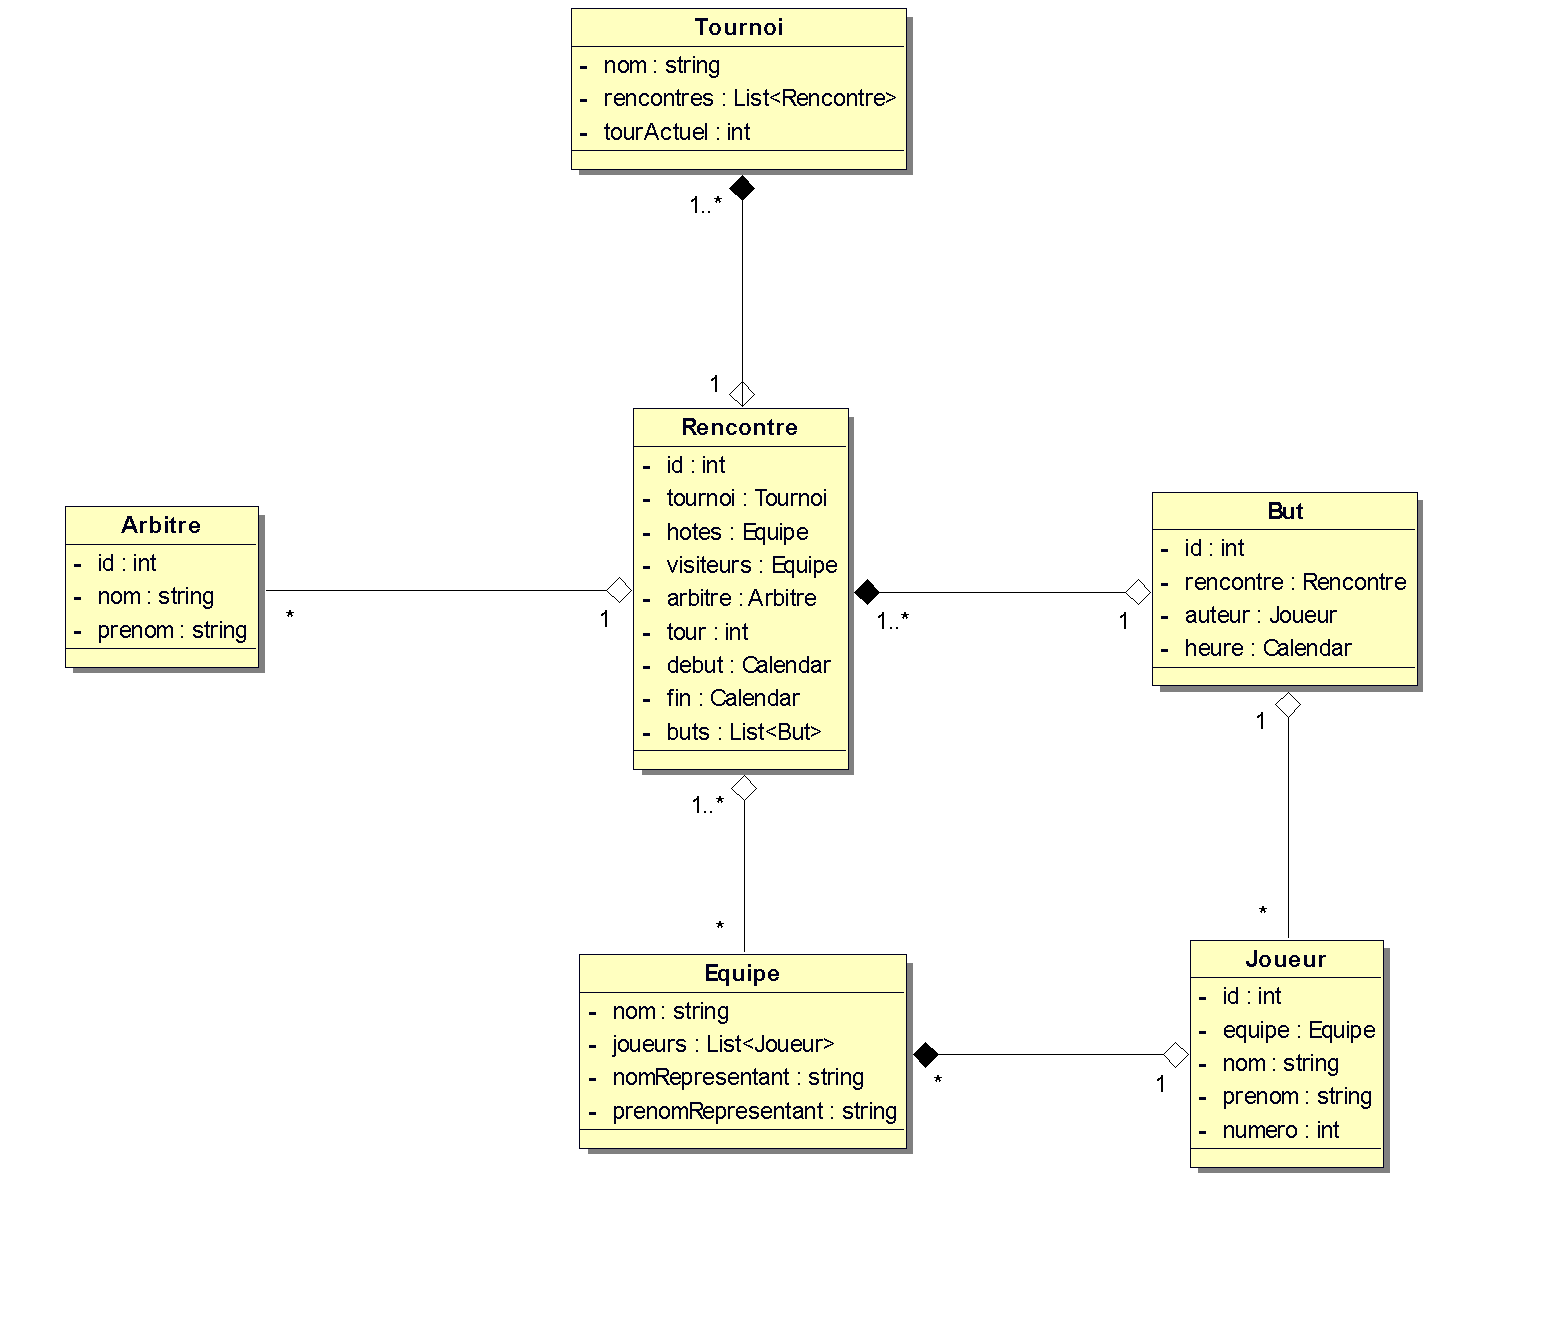
\includegraphics[scale=0.8]{class}}
	      \end{center}
	\legend{\underline{Diagramme de classes du modèle}}
	\end{figure}
blabla

\newpage
\subsection{Les EJB}

Le schéma ci-dessous représente le diagramme de classes de l'EJB Utilisateur créé.
\\
	\begin{figure}[hp]
	      \begin{center}
		\fbox{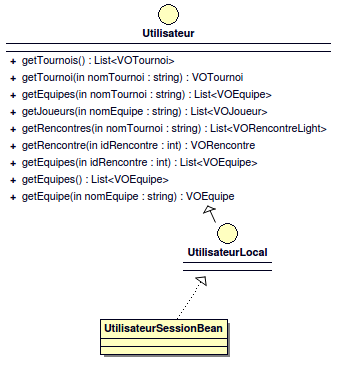
\includegraphics[scale=0.7]{ejb_u}}
	      \end{center}
	\legend{\underline{Diagramme de classes de l'EJB Utilisateur}}	
	\end{figure}
\\

L'EJB Utilisateur se compose de deux interfaces (\textit{Utilisateur} et \textit{UtilisateurLocal}) et d'une classe d'implémentation (\textit{UtilisateurSessionBean}). L'interface \textit{Utilisateur} définit les profils des méthodes implémentées par la classe \textit{UtilisateurSessionBean}. L'interface \textit{UtilisateurLocal} correspond à l'interface locale de l'EJB utilisée par la facade de notre application. L'ensemble des méthodes définies dans cet EJB retournent un Value Object ou une liste de Value Objects. En effet, l'utilisateur ne doit pas être en mesure de connaitre l'ensemble des attributs et méthodes des classes du modèle.

\newpage
Le schéma ci-dessous représente le diagramme de classes de l'EJB Administrateur créé.
\\
	\begin{figure}[hp]
	      \begin{center}
		\fbox{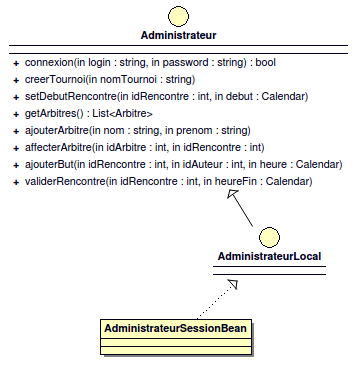
\includegraphics[scale=0.7]{ejb_a}}
	      \end{center}
	\legend{\underline{Diagrammes de classes de l'EJB Administrateur}}	
	\end{figure}
\\

L'EJB Administrateur se compose de deux interfaces (\textit{Administrateur} et \textit{AdministrateurLocal}) et d'une classe d'implémentation (\textit{AdministrateurSessionBean}). L'interface \textit{Administrateur} définit les profils des méthodes implémentées par la classe \textit{AdministrateurSessionBean}. L'interface \textit{AdministrateurLocal} correspond à l'interface locale de l'EJB utilisée par la facade de notre application. Les méthodes définies concernent la connexion de l'administrateur à l'application, la création d'un tournoi ou encore le déroulement des matchs (indication des horaires, affectation des arbitres).

\newpage
Le schéma ci-dessous représente le diagramme de classes de l'EJB Représentant créé.
\\
	\begin{figure}[hp]
	      \begin{center}
		\fbox{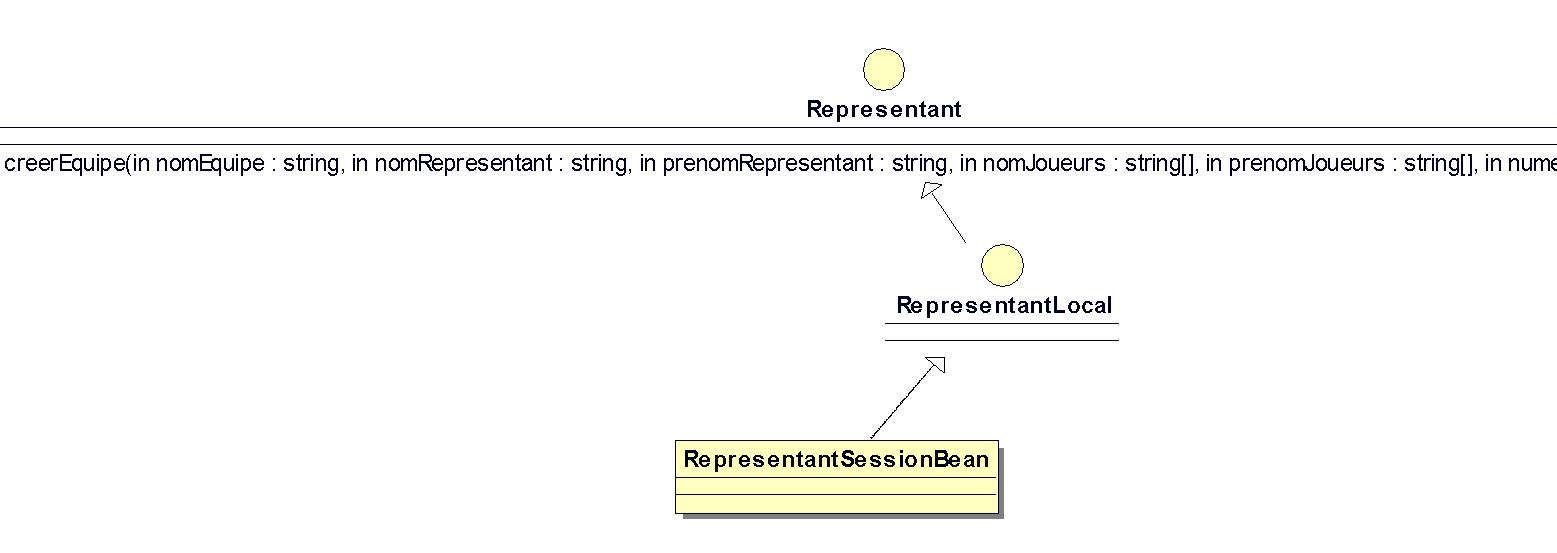
\includegraphics[scale=0.8]{ejb_r}}
	      \end{center}
	\legend{\underline{Diagramme de classes de l'EJB Représentant}}
	\end{figure}
\\
	
L'EJB Représentant se compose de deux interfaces (\textit{Representant} et \textit{RepresentantLocal}) et d'une classe d'implémentation (\textit{RepresentantSessionBean}). L'interface \textit{Representant} définit le profil de la méthode implémentée par la classe \textit{RepresentantSessionBean}. L'interface \textit{RepresentantLocal} correspond à l'interface locale de l'EJB utilisée par la facade de notre application. La méthode définie consiste à la création d'une équipe au sein de l'application.

\newpage
Le schéma ci-dessous représente le diagramme de classes de l'EJB session Facade créé.
\\
	\begin{figure}[hp]
	      \begin{center}
		\fbox{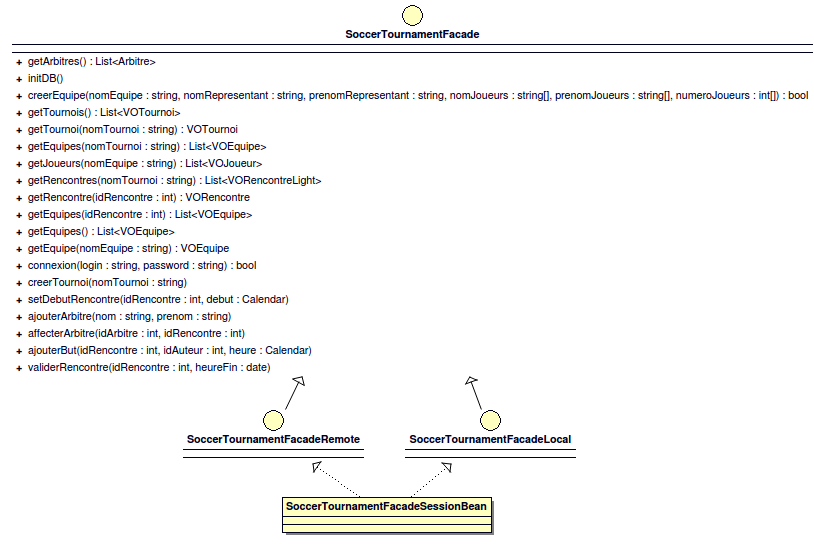
\includegraphics[scale=0.7]{ejb_f}}
	      \end{center}
	\legend{\underline{Diagramme de l'EJB session Facade}}
	\end{figure}	
\\

L'EJB session Facade se compose de trois interfaces (\textit{SoccerTournamentFacade}, \textit{SoccerTournamentFacadeLocal} et \textit{SoccerTournamentFacadeRemote}) et d'une classe d'implémentation (\textit{SoccerTournamentFacadeBean}). L'interface \textit{SoccerTournamentFacadeLocal} correspond à l'interface locale de l'EJB utilisée dans notre application. Nous avons également créé l'interface \textit{SoccerTournamentFacadeRemote} dans le cas où nous devions atteindre la façade à distance. Cet EJB regroupe l'ensemble des méthodes définies dans les EJB créés ainsi qu'une méthode \textit{InitDB()} nous permettant d'initialiser la base de données au lancement de l'application. La base de données se charge ainsi, à l'aide de fichiers XML préalablement remplis. 

\newpage
\subsection{Les Value Objects}

Le schéma ci-dessous représente le diagramme de classes des Value Objects créés.
	\begin{figure}[here]
	      \begin{center}
		\fbox{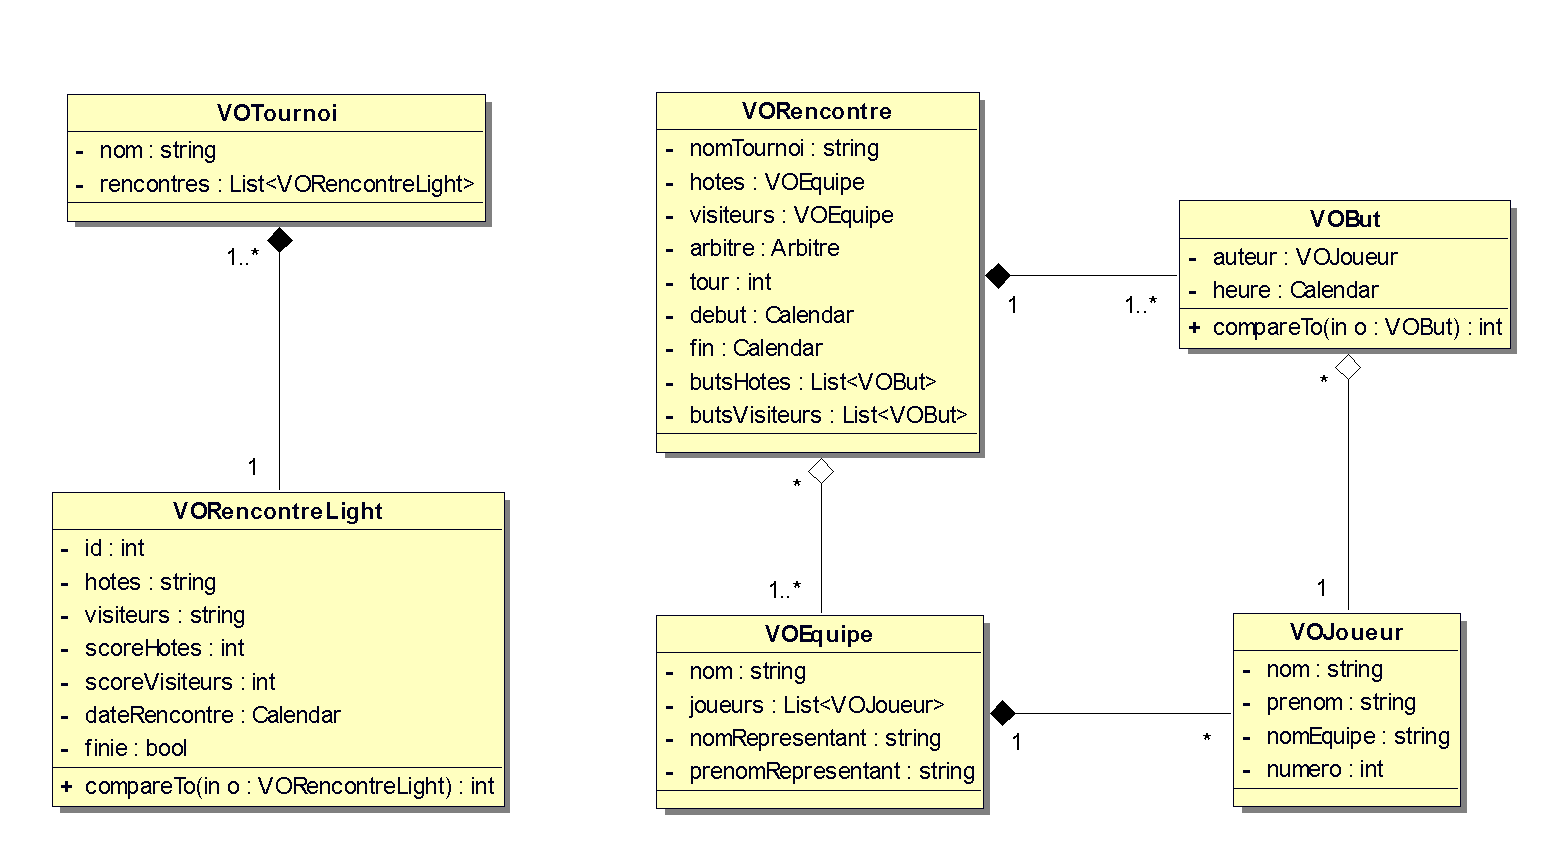
\includegraphics[scale=0.8]{vo}}
	      \end{center}
	\legend{\underline{Diagramme de classes des Value Objects}}
	\end{figure}
blabla

\newpage
\section{Diagramme de cas d'utilisation}
	\begin{figure}[hp]
	      \begin{center}
		\fbox{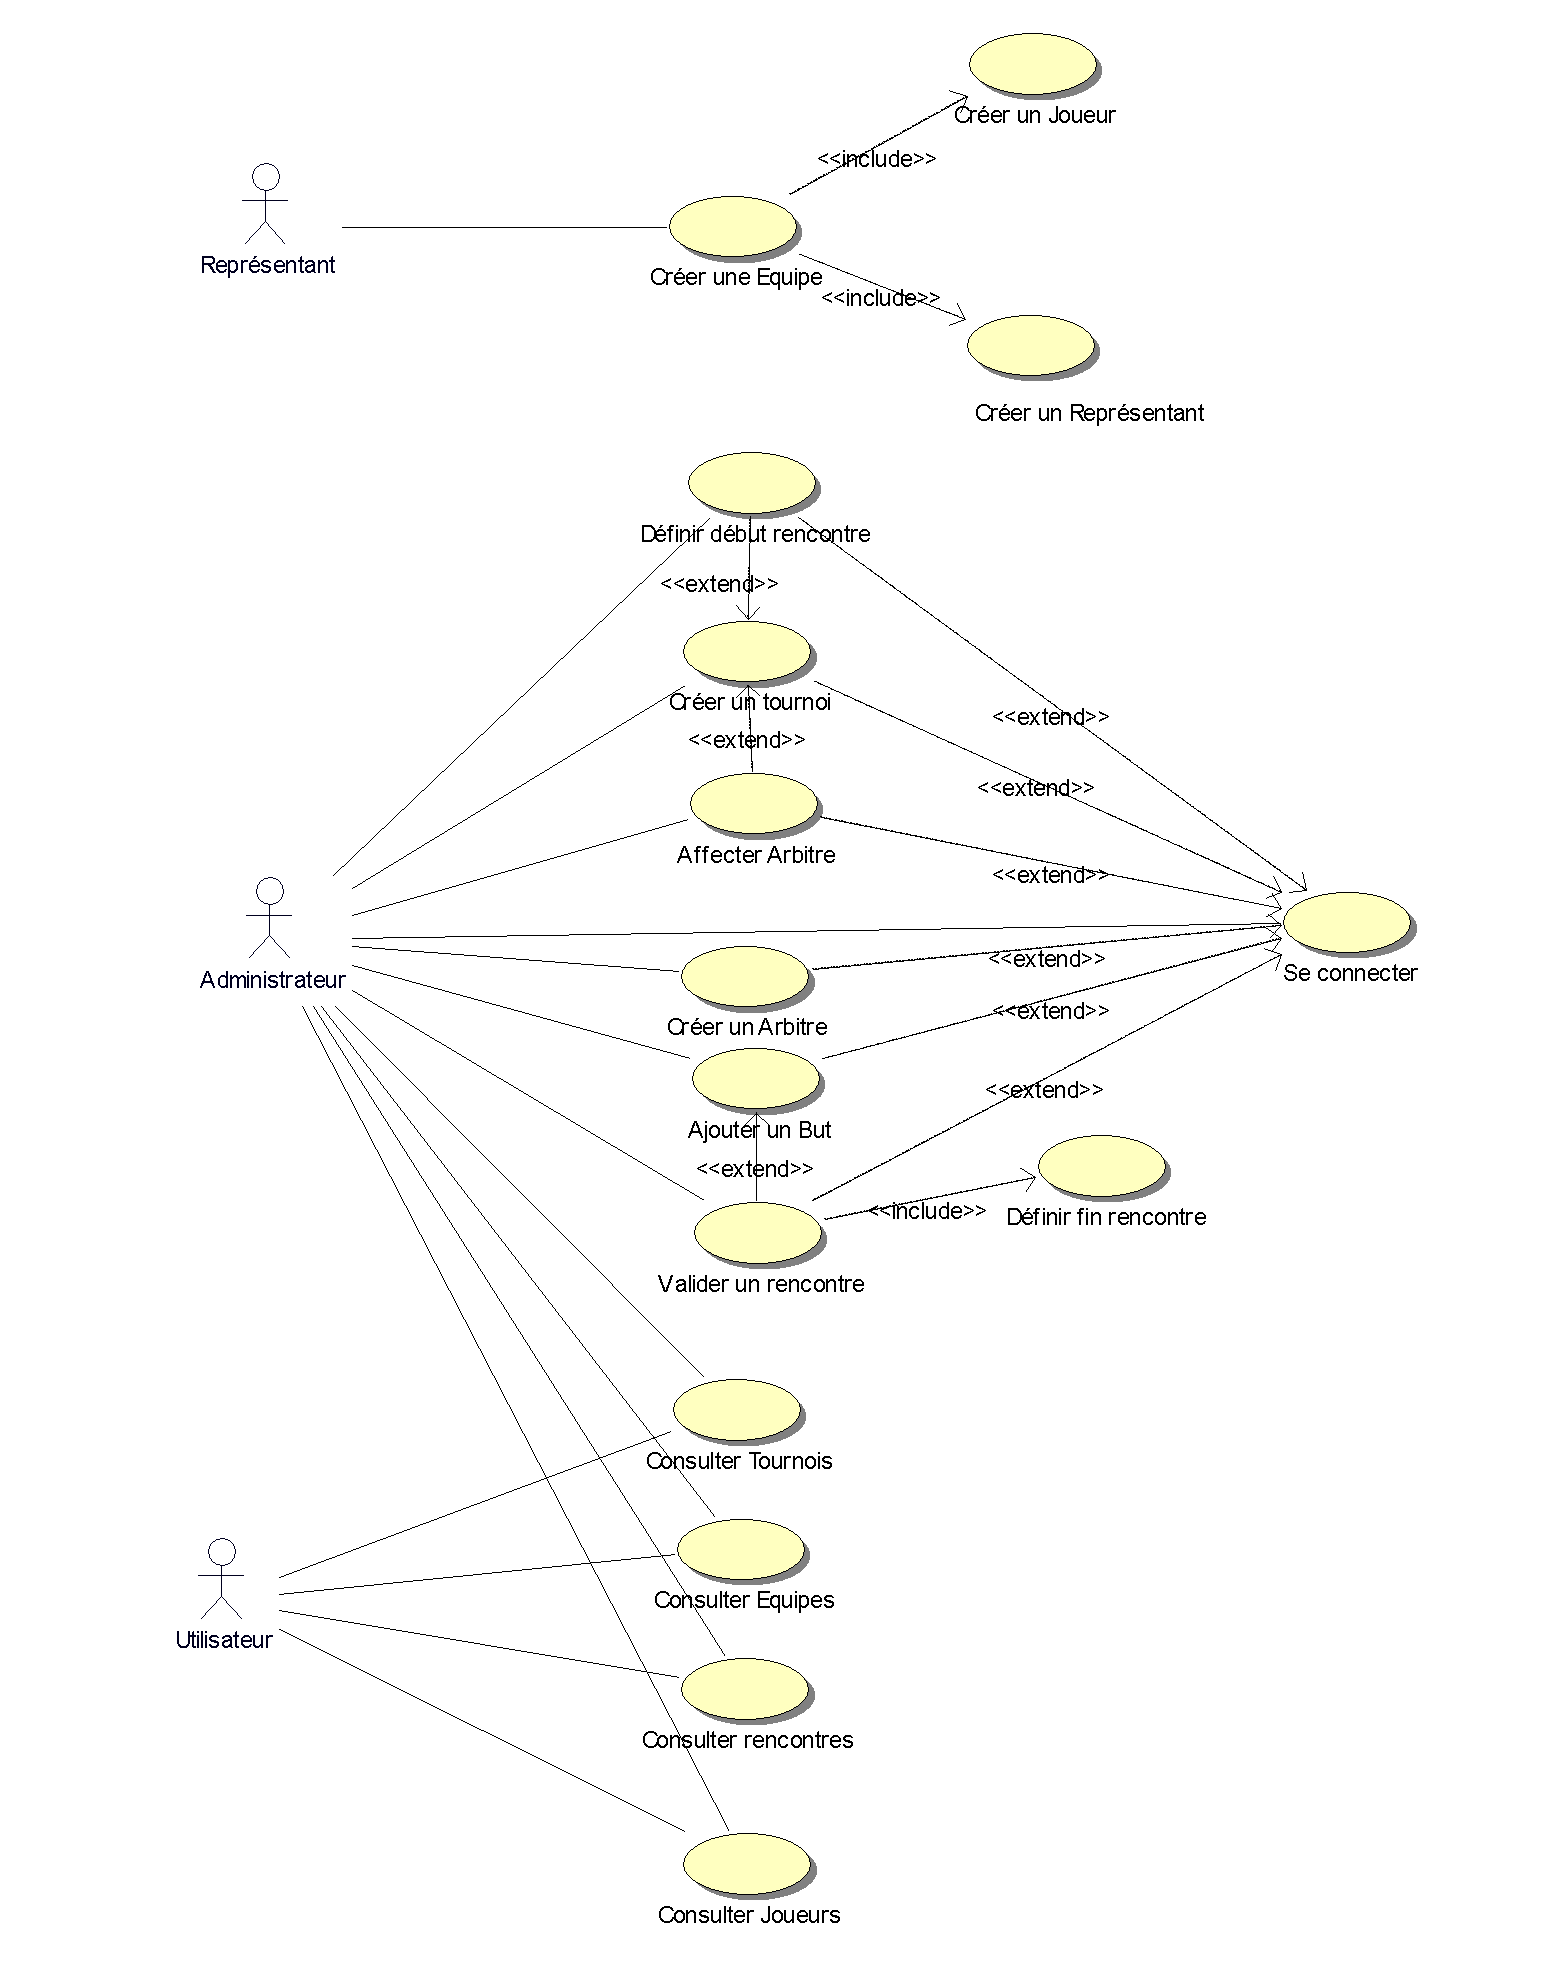
\includegraphics[scale=0.7]{use_cases}}
	      \end{center}
	\legend{\underline{Diagramme de cas d'utilisation}}
	\end{figure}
blabla

\newpage
\section{Schéma synthétique de l'application}
	\begin{figure}[hp]
	      \begin{center}
		\fbox{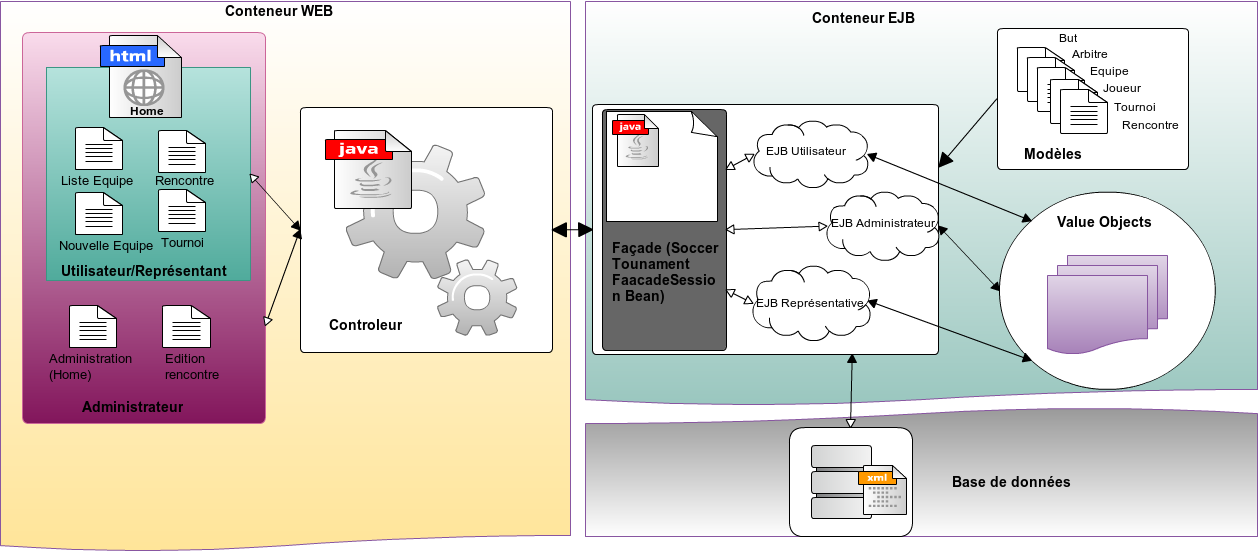
\includegraphics[width=18cm]{AAR}}
	      \end{center}
	\legend{\underline{Schéma synthétique de l'application}}
	\end{figure}
blabla

\newpage
\chapter{Répartition du travail}
\section{Gestion du temps de travail}

Le diagramme de Gantt ci-dessous présente la répartition du travail tout au long du projet.
\\
	\begin{figure}[hp]
	      \begin{center}
		\fbox{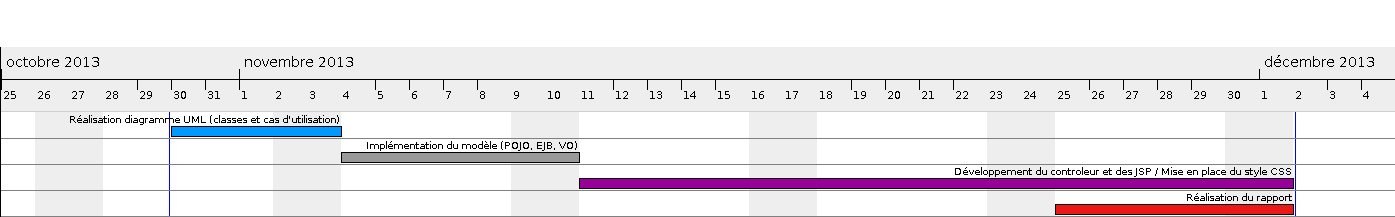
\includegraphics[width=18cm]{gantt}}
	      \end{center}
	\legend{\underline{Gestion du temps de travail}}
	\end{figure}
\\

La première semaine de travail fut consacrée à l'analyse UML et à l'élaboration des diagrammes de classes et des diagrammes de cas d'utilisation. Une fois cela fait, nous avons débuté l'implémentation du modèle de l'application à savoir les objets POJO, les EJB ainsi que les Value Objects. Le développpement du controleur et des vues utilisateurs et administrateurs a été réalisé ensuite jusqu'à la fin du projet. Le rapport, quant à lui, a été rédigé dans la dernière semaine de travail.

\section{Répartition des tâches}

\chapter{Guide d'utilisation}

\chapter*{Conclusion}

Ce projet aura permis de mettre en oeuvre les connaissances vues tout au long du semestre. Le groupe a pu améliorer ses compétences dans l'utilisation de la technologie Java EE et a acquis les principales notions de persistence d'objets, dans une base de données, avec l'usage des EJB. L'intérêt des Value Objects a été compris lors de ce projet et, les membres du groupe ont également renforcés leurs compétences dans le domaine du Web en travaillant sur un controleur et ses JSP. 

\end{document}
